\section{Auswertung}
\label{sec:Auswertung}
Der Versuch wird, wie in \autoref{sec:Durchführung} aufgebaut und durchgeführt.
\subsection{Bestimmung der Weglänge}
\label{subsec:Weglänge}
Im Folgenden wird die mittlere Weglänge bei verschiedenen Temperaturen bestimmt. Dazu wird mit \autoref{eqn:psät} der Sättigungsdampfdruck $p_{sät}$ bei den gemessenen 
Temperaturen bestimmt. Danach wird $\bar{\omega}$ mit der \autoref{eqn:Weglänge} bestimmt. Alle Werte werden in die \autoref{tab:Weglänge} eingetragen.
\begin{table}[H]
  \centering
  \caption{Gemsesene und bestimmte Werte für die Wellenlänge.}
  \label{tab:Wellenlänge}
  \sisetup{table-format=2.2}
  \begin{tabular}{S[table-format=3.2] S[table-format=2.3] S[table-format=1.4] S[table-format=1.4]}
  \toprule
  {Temperaturen $T / \si{\kelvin}$} & {Sättigungsdampfdruck $p_{sät} / \si{\milli\bar}$} & {mittlere Weglänge $\bar{\omega} / \si{\centi\meter}$} & {Verhältnis $\frac{a/\bar{\omega}}$}\\
  \midrule
    296.45   & 0.005 & 0.6241 &   \\
    416.15  & 3.669 & 0.0008  &  \\
    442.15  & 9.695 & 0.0003  &  \\
    452.15  & 13.674 & 0.0002 &   \\
  \bottomrule
  \end{tabular}
\end{table}
T =  [296.45 416.15 442.15 452.15]
psät=  [4.64657855e-03 3.66913288e+00 9.69451481e+00 1.36740660e+01]
w =  [6.24115136e-01 7.90377480e-04 2.99138230e-04 2.12080298e-04]
%Ende der Weglänge

\subsection{Integrale und differentielle Energieverteilung}
\label{subsec:Energieverteilung}

Tiefpunkt für $T_1$ bei $\qty{8.25}{\volt}$ und $T_2$ bei $\qty{1.29}{\volt}$.

%Ende der Energieverteilung

\subsection{Franck-Hertz-Kurve} % (fold)
\label{sub:Franck-Hertz-Kurve}



% subsection Franck-Hertz-Kurve (end)

\begin{figure}
  \centering
  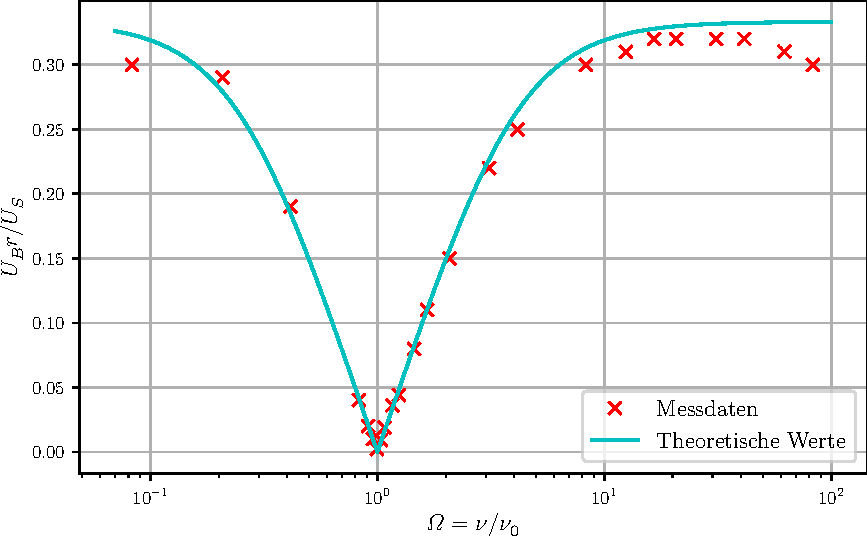
\includegraphics{plot.pdf}
  \caption{Plot.}
  \label{fig:plot}
\end{figure}



